\documentclass{beamer}

\usepackage[utf8]{inputenc}
\usecolortheme{beaver}
\usepackage{caption}
\usepackage{subcaption}
\usepackage{mathtools}
\usepackage{todonotes}
\usepackage{amsmath}
\usepackage{bm}
\usepackage{listings}
\usepackage{ragged2e}
\usepackage{fancyvrb}

\def\ci{\perp\!\!\!\!\!\perp}

\newtheorem{proposition}{Proposition}

\setbeamertemplate{section in toc}{\inserttocsectionnumber.~\inserttocsection}
\usetheme{Boadilla}
\makeatletter
\setbeamertemplate{footline}{%
    \leavevmode%
    \hbox{%
        \begin{beamercolorbox}[wd=.3\paperwidth,ht=2.25ex,dp=1ex,center]{author in head/foot}%
            \usebeamerfont{author in head/foot}\insertshortauthor\expandafter\beamer@ifempty\expandafter{\beamer@shortinstitute}{}{~~(\insertshortinstitute)}
        \end{beamercolorbox}%
        \begin{beamercolorbox}[wd=.55\paperwidth,ht=2.25ex,dp=1ex,center]{title in head/foot}%
            \usebeamerfont{title in head/foot}\insertshorttitle
        \end{beamercolorbox}%
        \begin{beamercolorbox}[wd=.15\paperwidth,ht=2.25ex,dp=1ex,right]{date in head/foot}%
            \usebeamerfont{date in head/foot}\insertshortdate{}\hspace*{2em}
            \insertframenumber{} / \inserttotalframenumber\hspace*{2ex} 
        \end{beamercolorbox}}%
        \vskip0pt%
    }
\makeatother

\begin{document}

\title[Unified CI test for Ordinal and Categorical Variables]{A Simple Unified Approach to Testing High-Dimensional Conditional Independencies for Ordinal and Categorical Variables}
\author {Ankur Ankan \and Johannes Textor}
\institute[]{Radboud University, Netherlands}
\date{}
\maketitle

\begin{frame}
	\frametitle{Overview}
	\tableofcontents
\end{frame}

\section{Motivation/Applications}
\begin{frame}
	\begin{center} \Huge{Motivation/Applications} \end{center}
\end{frame}
\begin{frame}
	\frametitle{Directed Acyclic Graphs}
	\begin{block}{Causal Markov Condition}
		Every node in the DAG is conditionally independent of its non-descendants, given its parents.
	\end{block}
	\begin{figure}
		\centering
		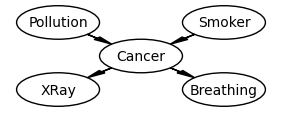
\includegraphics[scale=0.6]{imgs/example_dag.png}
		\caption*{An example of Directed Acyclic Graph (DAG) \footnotemark}
	\end{figure}
	In the DAG shown above,
	\begin{equation*}
		\begin{split}
			\text{\emph{XRay}} \ci & \text{\emph{Pollution}} | \text{\emph{Cancer}} \\
			\text{\emph{Breathing}} \ci & \text{\emph{Smoker}} | \text{\emph{Cancer}} \\
			& \vdots \\
		\end{split}
	\end{equation*}
	\footnotetext[1]{\footnotesize{K. B. Korb, A. E. Nicholson. Bayesian Artificial Intelligence}}
\end{frame}

\begin{frame}[fragile]
	\frametitle{Model Testing}
	\begin{itemize}
		\item In applied research, most of the DAGs are constructed by hand
			based on domain knowledge.
		\item Important to test whether the theorized model is consistent with data.
		\item Conditional Independence (CI) tests can be used to verify whether the implied
			CIs of the model are valid in the data.
	\end{itemize}

	\begin{figure}
		\centering
 		\begin{BVerbatim}
		             x2 df    p.value
Brth _||_ Pllt | Cncr 4.7571803  2 0.09268115
Brth _||_ Smkr | Cncr 9.0058063  2 0.01107679
Brth _||_ XRay | Cncr 1.9104270  2 0.38472999
 		\end{BVerbatim}
		\caption*{Example model testing output from R package \emph{dagitty}}
	\end{figure}
\end{frame}

\begin{frame}
	\frametitle{Structure Learning}
	\begin{itemize}
		\setlength\itemsep{1em}
		\item CI implies that no direct causal link exists between the variables. \newline
			$ \text{\emph{XRay}} \ci \text{\emph{Smoker}} | \text{\emph{Cancer}} \implies \text{No edge b/w \emph{XRay} and \emph{Smoker}} $

		\item Constraint-Based structure learning algorithms like PC
			and FCI use CI tests to systematically search for CIs
			in the dataset to determine model skeletons.
	\end{itemize}
	\begin{figure}
		\centering
		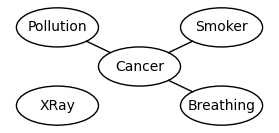
\includegraphics[scale=0.6]{imgs/example_sl.png}
		\caption*{Structure Learning Example}
	\end{figure}
\end{frame}

\section{Background}
\begin{frame}
	\begin{center} \Huge{Background} \end{center}
\end{frame}
\begin{frame}
	\frametitle{(Conditional) Independence}
	\begin{block}{Independence}
		Two random variables $ X $ and $ Y $ are independent,
		$ X \ci Y $ if and only if $ P(X, Y) = P(X) \cdot P(Y) $.
	\end{block}
	\vspace{1em}

	\begin{block}{Conditional Independence}
		Two random variables $ X $ and $ Y $ and are said to be
		conditionally independent given $ \bm{Z} $, $ X \ci Y | \bm{Z}
		$ if and only if for all $ z $ with $ p(z) > 0 $, $ P(X, Y |
		Z=z) = P(X | Z=z) \cdot P(Y | Z=z) $
	\end{block}
\end{frame}

\begin{frame}
	\frametitle{CI Testing is Difficult}
	\begin{figure}
		\centering

		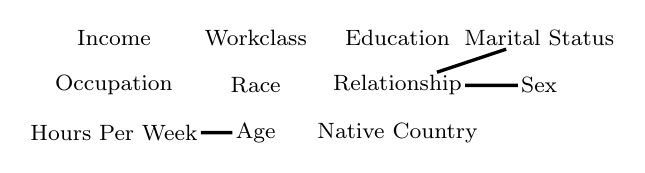
\begin{tikzpicture}[scale=0.6]
		\tikzstyle{every node}=[align=center, inner sep=1pt]
		\node at (0,0) {\footnotesize Income};
		\node at (3,0) {\footnotesize Workclass};
		\node at (6,0) {\footnotesize Education};
		\node (mrts) at (9 ,0) {\footnotesize Marital~Status};
		
		\node at (0,-1) {\footnotesize Occupation};
		\node (rltn) at (6,-1) {\footnotesize Relationship};
		\node at (3,-1) {\footnotesize Race};
		\node (sex) at (9,-1) {\footnotesize Sex};
		
		\node (hrpw) at (0,-2) {\footnotesize Hours~Per~Week};
		\node at (6,-2) {\footnotesize Native~Country};
		\node (age) at (3,-2) {\footnotesize Age};
		\draw [very thick] (sex) -- (rltn);
		\draw [very thick] (mrts) -- (rltn);
		\draw [very thick] (hrpw) -- (age);
		\end{tikzpicture}
		\caption*{Learned structure for US census income dataset using chi-square test}
	\end{figure}
	\begin{itemize}
		\item Testing for CI is much harder compared to testing for
			non-conditional independence.
		\item Especially in case of high cardinality or high number of
			conditional variables.
		\item In the continuous case, no test can exist which is calibrated and
			has power over all distributions where CI is True. \footnotemark
		\item Many different approaches and tests have been proposed.
	\end{itemize}

	\footnotetext[2]{\footnotesize{Shah, Rajen D., and Jonas Peters. "The hardness of conditional independence testing and the generalised covariance measure." The Annals of Statistics, 2020}}
\end{frame}

\begin{frame}
	\frametitle{Main Classes of Tests}
	\begin{enumerate}
		\setlength\itemsep{1em}
		\item Stratification based tests
		\item Variable Importance based tests
		\item Residulaization based tests
	\end{enumerate}
\end{frame}

\begin{frame}
	\frametitle{Stratification Based Tests}
	\begin{itemize}
		\setlength\itemsep{1em}
		\item Converts CI test into simple non-conditional independence test by splitting 
			the dataset such that conditional variables are constant in each stratum. \newline
			$$ D[X, Y, \bm{Z}] = \{ D[X, Y, \bm{Z}=\bm{z_1}], D[X, Y, \bm{Z}=\bm{z_2}], \cdots \} $$
		\item Runs non-conditional test on each stratum and combines the results.
		\item Most common type of test for discrete variables. Examples
			are chi-square, G-test, mutual information based test,
			etc. 
		\item As the number or cardinality of conditional variables is
			increased, exponentially less data is available in each
			stratum, resulting in it loosing power.
	\end{itemize}
\end{frame}

% \begin{frame}
% 	\frametitle{Statification Based Test Example: Chi-squared}
% 	\begin{block}{}
% 	\begin{columns}
% 		\begin{column}{0.25 \textwidth}
% 			\begin{block}{\centering D}
% 			\begin{tabular}{c c c}
% 				X  & Y  & Z \\
% 				\hline
% 				X1 & Y1 & Z1 \\
% 				X1 & Y2 & Z2 \\
% 				X2 & Y1 & Z1 \\
% 				X3 & Y3 & Z2 \\
% 				\vdots & \vdots & \vdots \\
% 			\end{tabular}
% 			\end{block}
% 		\end{column}
% 		\begin{column}{0.25 \textwidth}
% 			\begin{block}{\centering $D_1$}
% 				\begin{tabular}{c c c}
% 					X & Y & Z \\
% 					\hline
% 					X1 & Y1 & Z1 \\
% 					X2 & Y1 & Z1 \\
% 					\vdots & \vdots & \vdots \\
% 				\end{tabular}
% 			\end{block}
% 			\begin{block}{\centering $ D_2 $}
% 				\begin{tabular}{c c c}
% 					X & Y & Z \\
% 					\hline
% 					X1 & Y2 & Z2 \\
% 					X3 & Y3 & Z2 \\
% 					\vdots & \vdots & \vdots \\
% 				\end{tabular}
% 			\end{block}
% 			\begin{block}{\centering $ D_i $}
% 			\end{block}
% 		\end{column}
% 		\begin{column}{0.5 \textwidth}
% 			\begin{block}{}
% 				$(X \ci Y)_{D_1} \to \chi_{D_1} $ and $ df_{D_1} $.
% 			\end{block}
% 			\begin{block}{}
% 				$(X \ci Y)_{D_2} \to \chi_{D_2} $ and $ df_{D_2} $.
% 			\end{block}
% 			\begin{block}{}
% 				$(X \ci Y)_{D_i} \to \chi_{D_i} $ and $ df_{D_i} $.
% 			\end{block}
% 		\end{column}
% 	\end{columns}
% 	\end{block}
% 	\begin{block}{}
% 		\centering
% 		$ (X \ci Y | Z)_{D} \to \sum_i \chi_{D_i} $ and $ df_{D} = \sum_i df_{D_i} $
% 	\end{block}
% \end{frame}

% \begin{frame}
% 	\frametitle{Stratification Based Tests: Advantages/Disadvantages}
% 	\begin{itemize}
% 		\item As the number of conditional variables is increased, exponentially
% 			less data is available in each stratum.
% 		\item Looses power when number of conditonal variables
% 			are increased.
% 	\end{itemize}
% \end{frame}

\begin{frame}
	\frametitle{Variable Importance Tests}
	\begin{itemize}
		\setlength\itemsep{1em}
		\item Based on comparing the probability models: $\hat{p}(x |
			y, z) $ and $ \hat{p}(x | z) $. 
		\item The idea being that if adding the additional variable to
			the predictors doesn't improve the fit, the varible
			doesn't have any extra infromation.  E.g. Stochastic
			Complexity-Based Conditional Independence Test (SCCI)
			\footnotemark.
		\item The two probability models are trained and some goodness of fit is compared.
		\item Can utilize any statistical model for which a reasonable goodness
			of fit exist.
		\item Main disadvantage is that these tests are inherently
			asymmetrical i.e. the result of $ X \ci Y | Z $ can be
			different from $ Y \ci X | Z $.
	\end{itemize}
	\footnotetext[3]{\footnotesize Marx, Alexander, and Jilles Vreeken. "Testing conditional independence on discrete data using stochastic complexity." PMLR, 2019}

\end{frame}

% \begin{frame}
% 	\frametitle{Variable Importance Test Example: SCCI}
% 	\begin{itemize}
% 		\item Given random variables $ X $, $Y $, and $Z$,
% 			$$ S(X | Z ) - S(X|Z, Y) \le 0 \implies (X \ci Y | Z) $$
% 		\item $ S $ is the conditional stochastic complexity measure defined using normalized maximum likelihood.
% 	\end{itemize}
% \end{frame}

% \begin{frame}
% 	\frametitle{Variable Importance Tests: Advantages/Disadvantages}
% 	\begin{itemize}
% 		\item Can utilize any statistical model for which a reasonable goodness
% 			of fit exist.
% 		\item Inherently asymmetrical. For example, in the case of SCCI
% 			the value of $ S(X | Z) - S(X|Y,Z) $ can be different
% 			from $ S(Y|Z) - S(Y|X, Z) $, the result of $ X \ci Y |
% 			Z $ can be different from $ Y \ci X | Z $.
% 	\end{itemize}
% 
% \end{frame}

\begin{frame}
	\frametitle{Residualization Based Tests}
	\begin{itemize}
		\setlength\itemsep{1em}
		\item Uses two estimators $ \mathbb{E}[X| Z] $ and $
			\mathbb{E}[Y | Z] $ and checks for the multiplicative
			association between the residuals. E.g.
			Partial Correlation test, generalized covariance measure etc.
		\item Relies on the theorem from Daudin [1980] \footnotemark 
			that under CI, if the estimators have ``valid'' residuals
			such that $ \mathbb{E}[R_{X|Z}] = \mathbb{E}[R_{Y|Z}] = 0 $,
			then $ \mathbb{E}[R_{X|Z} R_{Y|Z}] = 0 $.
		\item Any estimator can be used as long as it has ``valid'' residuals.
		\item No easy way to define residuals for ordinal and categorical variables.
	\end{itemize}
	\footnotetext[4]{\footnotesize Daudin, J. J. "Partial association measures and an application to qualitative regression." Biometrika, 1980}
\end{frame}

% \begin{frame}
% 	\frametitle{Residualization Based Test Example: Partial-correlation}
% 	\begin{itemize}
% 		\item Train two linear regression models
% 			$$ E_1 = X \sim Z \; \; \; \; \; \; \; E_2 = Y \sim Z $$
% 		\item Predict $ X $ and $ Y $ using the estimators 
% 			$$ \hat{X} = E_1(Z) \; \; \; \; \; \; \; \hat{Y} = E_2(Z) $$
% 		\item Compute the residuals
% 			$$ R_X = X - \hat{X} \; \; \; \; \; \; \; R_Y = Y - \hat{Y} $$
% 		\item Use Pearson correlation test on $ R_X $ and $ R_Y $.
% 	\end{itemize}
% \end{frame}

% \begin{frame}
% 	\frametitle{Residualization Based Tests: Advantages/Disadvantages}
% 	\begin{itemize}
% 		\item Any estimator can be used as long as it has ``valid'' residuals.
% 		\item No easy way to define residuals for ordinal and categorical variables.
% 		\item No residualization based test exists for categorical or ordinal variables.
% 	\end{itemize}
% \end{frame}

\section{Proposed Unified Test}
\begin{frame}
	\begin{center} \Huge{Proposed Unified Test for Ordinal and Categorical Data} \end{center}
\end{frame}
\begin{frame}
	\frametitle{Unified test for all data types}
	\begin{itemize}
		\setlength\itemsep{1em}
		\item Residualization based approach.
		\item Uses Li-Shepherd (LS) residuals \footnotemark.
		\item Any unbiased estimator can be used.
		\item Empirical results shown using Logistic Regression (GLM) and Random Forest (RFT).
	\end{itemize}
	\footnotetext[5]{\footnotesize C. Li and B. E. Shepherd. "A new residual for ordinal outcomes." Biometrika, 2012}
\end{frame}


\begin{frame}
	\frametitle{Residual for ordinal variables: LS-Residuals}
	\begin{block}{LS-Residuals}
	Given an ordinal variable $ Y $ and an estimate $ \hat{p}(y) $ of $
	p(y) $, LS-Residual for sample $ y_i $ is defined as:
	$$ R_{y_i} = \hat{p}(Y < y_i) - \hat{p}(Y > y_i) $$
	\end{block}

	For the binary case with $ Y \in \{0, 1\} $:
	$$ R_{y_i} = y_i - \hat{p}(Y = 1) $$

	For the conditional case for sample $ (y|z)_i $,
	$$ R_{y_i | z_i} = \hat{p}(Y < y_i | Z=z_i) - \hat{p}(Y>y_i|Z=z_i) $$

\end{frame}

% \begin{frame}
% 	\frametitle{Residual for ordinal variables: LS-Residuals Example}
% 	\begin{block}{Ordinal Variable}
% 		\vspace{1em}
% 			$ \hat{p}(y) = \begin{array}{llll} Y_0 & Y_1 & Y_2 & Y_3 \\ 0.1 & 0.3 & 0.5 & 0.1 \end{array} $
% 		\begin{itemize}
% 			\item If $ y = Y_2 $, $ R_{y} = \hat{p}(Y < Y_2) - \hat{p}(Y > Y_2) = 0.3 $
% 			\item If $ y = Y_3 $, $ R_{y} = \hat{p}(Y < Y_3) - \hat{p}(Y > Y_3) = 0.9 $
% 		\end{itemize}
% 	\end{block}
% 	\begin{block}{Binary Variable}
% 		$\hat{p}(Y) = \begin{array}{ll} Y_0 & Y_1 \\ 0.3 & 0.7 \end{array} $
% 		\begin{itemize}	
% 			\item If $ y = Y_0 $, $ R_{y} = Y_0 - \hat{p}(Y=1) = -0.7 $
% 			\item If $ y = Y_1 $, $ R_{y} = Y_1 - \hat{p}(Y=1) = 0.3 $
% 		\end{itemize}
% 	\end{block}
% \end{frame}

\begin{frame}
	\frametitle{Residual for Ordinal Variables: LS-Residual Example}
	For ordinal variable:
	\[
		\begin{array}{ccc}
			\bm{y} & \hat{p}(\bm{y}) & R_{y} \\

			\begin{bmatrix}
				Y_2 \\
				Y_3 \\
				Y_1 \\
				\vdots
			\end{bmatrix} &
			\begin{bmatrix}
				0.1 & 0.3 & 0.5 & 0.1 \\
				0.2 & 0.3 & 0.2 & 0.3 \\
				0.4 & 0.2 & 0.2 & 0.2 \\
				\vdots & \vdots & \vdots & \vdots
			\end{bmatrix} &
			\begin{bmatrix}
				\hat{p}(Y < Y_2) - \hat{p}(Y>Y_2) = 0.3 \\
				\hat{p}(Y < Y_3) - \hat{p}(Y>Y_3) = 0.9 \\
				\hat{p}(Y < Y_1) - \hat{p}(Y>Y_1) = 0 \\
				\vdots
			\end{bmatrix} \\
		\end{array}
	\]

	For categorical variable:
	\[
		\begin{array}{ccc}
			\bm{y} & \hat{p}(\bm{y}) & R_{\bm{y}} \\
			\begin{bmatrix}
				Y_3: & 0 & 0 & 0 & 1 \\
				Y_1: & 0 & 1 & 0 & 0 \\
				Y_2: & 0 & 0 & 1 & 0 \\
				\vdots & \vdots & \vdots & \vdots \\
			\end{bmatrix} & 
			\begin{bmatrix}
				0.1 & 0.3 & 0.5 & 0.1 \\
				0.2 & 0.3 & 0.2 & 0.3 \\
				0.4 & 0.2 & 0.2 & 0.2 \\
				\vdots & \vdots & \vdots & \vdots \\
			\end{bmatrix} & 
			\begin{bmatrix}
				-0.1 & -0.3 & 0.5 & -0.1 \\
				-0.1 & 0.7 & -0.5 & -0.1 \\
				-0.4 & -0.2 & 0.8 & -0.2 \\
				\vdots & \vdots & \vdots & \vdots \\
			\end{bmatrix} \\
		\end{array}
	\]
\end{frame}

\begin{frame}
	\frametitle{Test Statistic: Both ordinal variables}
	\begin{proposition}
	$$ Q_1(\bm{x}, \bm{y}) = \frac{1}{n} \frac{(R_{\bm{x}} \cdot R_{\bm{y}})^2}{\bm{var}(R_{\bm{x}} R_{\bm{y}})} $$
		\begin{center} If $ X \ci Y | Z $, asymptotically $ Q_1(\bm{x}, \bm{y}) \sim \chi^2(1) $. \end{center}
	\end{proposition}
	\begin{center}
		\begin{itemize}
			\item $ R_{\bm{x}} $ and $ R_{\bm{y}} $ are vectors of residuals.
			\item Square root of Generalized Covariance Measure (GCM) proposed by Shah and Peters (2020)
		\end{itemize}
	\end{center}
\end{frame}

\begin{frame}
	\frametitle{Test Statistic: One categorical and one ordinal}
	\begin{proposition}

		$$ Q_2(\bm{x}, \bm{y}) = \frac{1}{n} (d \times \hat{\Sigma}_d^{-1} \times d^T) $$
	where
	\begin{equation*}
		\begin{split}
		d &= (R_{\mathbb{I}(\mathbf{x}=1)} \cdot R_{\mathbf{y}}, \, \ldots \ , R_{\mathbb{I}(\mathbf{x}=k-1)} \cdot R_{\mathbf{y}}) \\ 
		\hat{\Sigma}_d &= Cov([R_\mathbb{I}(\mathbf{x}=1) \odot R_\mathbf{y}, \cdots, R_\mathbb{I}(\mathbf{x}=k-1) \odot R_\mathbf{y}])
		\end{split}
	\end{equation*}
		If $ X \ci Y | Z $, asymptotically $ Q_2(\bm{x}, \bm{y}) \sim \chi^2(k-1) $.
	\end{proposition}
	\begin{center}
		\begin{itemize}
			\item $ R_{\bm{x}} $ is a matrix of residuals with each column corresponding to a dummy state and $ R_{\bm{y}} $ is still a vector.
			\item One of the columns of the dummy encoded variable
				is dropped as it will be colinear. Including it will
				result in a non full-rank covariance matrix.
		\end{itemize}
	\end{center}
\end{frame}

\begin{frame}
	\frametitle{Test Statistic: Both categorical}
	\begin{proposition}

	$$ Q_3(\bm{x}, \bm{y}) = \frac{1}{n} (d \times \hat{\Sigma}_d^{-1} \times d^T) $$

	where
	\begin{equation*}
		\begin{split}
		d = (&R_{\mathbb{I}(\mathbf{x}=1)} \cdot R_{\mathbb{I}(\mathbf{y}=1)}, \, \ldots \ ,
				R_{\mathbb{I}(\mathbf{x}=k-1)} R_{\mathbb{I}(\mathbf{y}=1)}, \, \ldots \, , \\
		     &R_{\mathbb{I}(\mathbf{x}=1)} \cdot R_{\mathbb{I}(\mathbf{y}=r-1)}, \, \ldots \ ,
				R_{\mathbb{I}(\mathbf{x}=k-1)} R_{\mathbb{I}(\mathbf{y}=r-1)}) 
		\end{split}
	\end{equation*}
	\begin{equation*}
		\hat{\Sigma}_d = Cov([R_\mathbb{I}(\mathbf{x}=1) \odot R_\mathbb{I}(\mathbf{y}=1), \cdots, R_\mathbb{I}(\mathbf{x}=k-1) \odot R_\mathbb{I}(\mathbf{y}=r-1)])
	\end{equation*}

	If $ X \ci Y | Z $, asymptotically $ Q_3(\bm{x}, \bm{y}) \sim \chi^2((k-1)(r-1)) $.
	\end{proposition}
	\begin{center}
		\begin{itemize}
			\item Both $ R_{\bm{x}} $ and $ R_{\bm{y}} $ are matrices of residuals.
		\end{itemize}
	\end{center}

\end{frame}

\begin{frame}
	\frametitle{Test Summary}
	Given a dataset, $ \mathbf{D} $ and a CI statement $ X \ci Y | \bm{Z} $:
	\begin{enumerate}
		\setlength\itemsep{1em}
		\item If $\mathbf{Z} = \emptyset $ , do a non-conditional chi-squared test.
		\item If either $ X $ or $ Y $ are non-binary categorical,
			dummy encode them.
		\item Train two probability estimators $ p_x = \bm{x} \sim \bm{z} $ and
			$ p_y = \bm{y} \sim \bm{z} $
		\item Make probability predictions using these two estimators 
			$ \hat{p}(\bm{x}) = p_x(\bm{z}) $ and $ \hat{p}(\bm{y}) = p_y(\bm{\bm{z}}) $.
		\item Use $ \hat{p}(\bm{x}) $, $ \hat{p}(\bm{y}) $, and $ D $ to compute LS-Residuals $ R_{\bm{x}|\bm{z}} $ and $ R_{\bm{y}|\bm{z}} $.	
		\item Compute test statistic and df using $ R_{\bm{x}|\bm{z}} $ and $ R_{\bm{y}|\bm{z}} $.
	\end{enumerate}
\end{frame}
% 
% \begin{frame}
% 	\frametitle{Proof: M-estimation theory}
% 	\justifying{Given a vector of parameters $ \bm{\theta} $, and a function $ \Psi_i(\bm{\theta}) = \Psi(Y_i, X_i, \bm{Z}_i; \bm{\theta}) $, such that the following conditions are satisfied.}
% 	\begin{enumerate}
% 		\item $ \bm{\theta} $ can be estimated using $ \sum_{i=1}^n \Psi_i(\bm{\theta}) = 0 $.
% 		\item $ \Psi_i $ doesn't depend on $ i $ or $ n $.
% 		\item $ \mathbb{E}[\Psi_i(\bm{\theta})] = 0 $
% 	\end{enumerate}
% 
% 	From m-estimation theory, if $ \Psi $ is suitably smooth, then as $ n \to \infty $,
% 
% 	$$ \sqrt{n}(\hat{\bm{\theta}} - \bm{\theta}) \to \mathcal{N}(0, V(\bm{\theta})) $$
% 	where 
% 	\begin{equation*}
% 		\begin{split}
% 			V(\bm{\theta}) &= A(\bm{\theta}^{-1}) B(\bm{\theta})[A(\bm{\theta})^{-1}]' \\
% 			A(\bm{\theta}) &= \mathbb{E} \left[ - \frac{\partial}{\partial \bm{\theta}} \Psi_i(\bm{\theta}) \right] \\ 
% 			B(\bm{\theta}) &= \mathbb{E}[\Psi_i(\bm{\theta}) \Psi_i(\bm{\theta})]'
% 		\end{split}
% 	\end{equation*}
% 
% \end{frame}
% 
% \begin{frame}
% 	\frametitle{M-Estimator and Delta method}
% 	\begin{block}{Delta Method}
% 		If there is a sequence of random variables $X_n$ satisfying $ \sqrt{n}[X_n - \theta] \rightarrow \mathcal{N}(0, \sigma^2) $, then
% 		$$ \sqrt{n}[g(X_n) - g(\theta)] \rightarrow \mathcal{N}(0, [g'(\theta)] \sigma^2 [g'(\theta)]')$$
% 	\end{block}
% 	\begin{block}{M-Estimator and Delta Method}
% 		Given a function $ g(\bm{\theta}) $ which is a smooth function of $ \bm{\theta} $, we have:
% 
% 		$$ \sqrt{n} \left[ g(\hat{\bm{\theta}}) - g(\bm{\theta}) \right] \to \mathcal{N} \left( 0, \left[ \frac{\partial}{\partial \bm{\theta}} g(\bm{\theta}) \right] V(\bm{\theta}) \left[ \frac{\partial}{\partial \bm{\theta}} g(\bm{\theta}) \right]' \right) $$
% 	\end{block}
% \end{frame}

\begin{frame}
	\frametitle{Proof Outline}
	\begin{itemize}
		\item Define parameters such that our test statistics can be written as M-Estimators.
		\item Define a function, $ g(\bm{\theta}) $ on the M-Estimator parameters, $ \bm{\theta} $ for each of the test statistics such that $ Q = (\sqrt{n}g(\bm{\theta}))^2 $.
		\item From M-Estimator theory and delta method, as $ \sqrt{n}(g(\hat{\bm{\theta}}) - g(\bm{\theta})) \to \mathcal{N}(0, \sigma^2) $.
		\item We show that $ g(\bm{\theta}) = 0 $, implying $ \sqrt{n}g(\hat{\bm{\theta}}) \rightarrow \mathcal{N}(0, \sigma^2) $
		\item As $ Q = (\sqrt{n}g(\bm{\theta}))^2 $, $ Q \rightarrow \chi^2 $.
	\end{itemize}

\end{frame}

\begin{frame}
	\frametitle{M-Estimator for the test statistic}
	\begin{itemize}
		\item Divide our parameter vector into $ 3 $ sets: $ \bm{\theta} = \{ \bm{\theta^\bm{X}}, \bm{\theta^\bm{Y}}, \bm{\theta^\bm{T}} \} $.
		\item $ \bm{\theta^\bm{X}} $ and $ \bm{\theta^\bm{Y}} $ stay the same for all test
			statistics:

			\begin{equation*}
			\Phi_i(\bm{\theta}) = \begin{cases}
				\frac{\partial}{\partial \bm{\theta}^{\bm{Y}}} l_Y (Y_i, \bm{Z}_i; \bm{\theta^{Y}}) \\
				\frac{\partial}{\partial \bm{\theta}^{\bm{X}}} l_X (X_i, \bm{Z}_i; \bm{\theta^{X}}) \\
				\end{cases}
			\end{equation*}

		\item $ l_X $ and $ l_Y $ are log-likelihood functions of the probability models $ P(X | \bm{Z}) $ and $ P(Y | \bm{Z}) $ with parameters $ \bm{\theta}^X $ and $ \bm{\theta}^Y $ respectively.
		\item We use this as a partial M-estimator for our test statistic and define $ \bm{\theta}^T $ for each of our test statistic.
	\end{itemize}
\end{frame}

\begin{frame}
	\frametitle{Proof: Both ordinal case}
	\begin{equation*}
		\begin{split}
			\bm{\theta}^T &= (\theta_1, \theta_2) \\
			\Psi (X_i, Y_i, \mathbf{Z}_i; \bm{\theta}^T) &= 
				\begin{cases}
					R_{y_i} R_{x_i} - \theta_1 \\
					(R_{y_i} R_{x_i})^2 - \theta_2
				\end{cases} \\
			g(\bm{\theta}) &= \frac{\theta_1}{\sqrt{\theta_2 - \theta_1^2}} \\
			Q_1 &= (\sqrt{n} g(\bm{\theta}))^2 \\
		\end{split}
	\end{equation*}

	\begin{itemize}
		\item As $ n \rightarrow \infty $, $ \sqrt{n} (g(\hat{\bm{\theta}}) - g(\bm{\theta})) \rightarrow \mathcal{N}(0, 1) $.
		\item As $ g(\bm{\theta}) = 0 $, $ \sqrt{n}(g(\hat{\bm{\theta}}) \rightarrow \mathcal{N}(0, 1) \implies Q_1 \rightarrow \chi^2(1) $
	\end{itemize}

\end{frame}

\begin{frame}
	\frametitle{Proof: One ordinal and one categorical case}
	\begin{equation*}
		\begin{split}
			& \bm{\theta}^T = (\bm{\theta_1}, \bm{\theta_2}) \\
			& \bm{\theta_1} = (\theta_1^1, \theta_1^2, \cdots, \theta_1^{k-1}) \\
			& \bm{\theta_2} = (\theta_2^{11}, \cdots, \theta_2^{1(k-1)}, \theta_2^{21}, \cdots, \theta_2^{2(k-1)}, \cdots, \theta_2^{(k-1) (k-1)}) \\
			& \Psi(X_i, Y_i, \mathbf{Z}_i; \bm{\theta}^T) = 
				\begin{cases}
					R_{{\mathbb{I}(x=j)}_i}.R_{y_i} - \theta_1^j \, \, \forall j \in \{ 1, \cdots, k-1 \} \\
					(R_{{\mathbb{I}(x=j)}_i}.R_{y_i} \times R_{{\mathbb{I}(x=k)}_i}.R_{y_i}) - \theta_{2}^{jk} \,\, \forall j, k \in \{ 1, \cdots, k-1 \} \\
				\end{cases} \\
			& g(\bm{\theta}) = \bm{\theta_1} \bm{\wedge}
		\end{split}
	\end{equation*}

	where:
\begin{equation*}
	\begin{split}
		\bm{\wedge} &= \bm{\Sigma}^{-\frac{1}{2}} \\
		\Sigma^{i,j} &= \mathbb{E}[(R_{\mathbb{I}(\mathbf{x}=i)}.R_\mathbf{y})(R_{\mathbb{I}(\mathbf{x}=j)}.R_\mathbf{y})] - \mathbb{E}[R_{\mathbb{I}(\mathbf{x}=i)}.R_\mathbf{y}] \mathbb{E}[R_{\mathbb{I}(\mathbf{x}=j)}.R_\mathbf{y}] \\
			    &= \theta_2^{ij} - \theta_1^{i} \theta_1^{j} \\
	\end{split}
\end{equation*} 
	\begin{itemize}
		\item $ \sqrt{n}g(\hat{\bm{\theta}}) \to \mathcal{N}(0, \mathbb{I}_{(k-1)}) \implies Q_2 \to \chi^2(k-1) $
	\end{itemize}
\end{frame}
% \begin{frame}
% 	\frametitle{Proof: One ordinal and one categorical case}
% 	\begin{itemize}
% 		\item $ g(\bm{\theta}) $ is again chosen such that $ Q_2 = (\sqrt{n} g(\bm{\theta}))^2 $
% 		\item Using 
% 	\end{itemize}
% \end{frame}

\section{Empirical Results}
\begin{frame}
	\begin{center} \Huge{Empirical Results} \end{center}
\end{frame}
\begin{frame}{Empirical Analysis}
	\begin{itemize}
		\item Analysis shown using two estimators Generalized Linear Models (GLM) and Random Forest (RFT).
		\item Even though RF is not an M-Estimator, we use it as a sensitivity analysis for non M-estimators.
		\item We compared our proposed test to 4 other tests:
			\begin{enumerate}
				\item Mutual Information based Test (MI)
				\item Monte Carlo Permutation Test (MC-MI)
				\item Stochastic Complexity based CI (SCCI)
				\item Jonckheere-Terpstra Test (JT) (Only for ordinal case)
			\end{enumerate}
		\item List of analyses:
			\begin{enumerate}
				\item Calibration
				\item Discrimination
				\item Model Testing
				\item Simulated data Strucutre Learning
				\item Read Dataset Structure Learning
				\item Runtime
			\end{enumerate}

	\end{itemize}
\end{frame}
\begin{frame}
	\frametitle{Empirical Analysis: Calibration}
	\begin{itemize}
		\item Under the null (i.e. $ X \ci Y | Z $), the p-value should
			be uniformly distributed.
		\item We test the distribution of p-values on simulated
			datasets with varying sample sizes and number of
			conditional variables.
		\item Conditionally Independent datasets are generated using the DAG:
			\begin{figure}
				\centering
				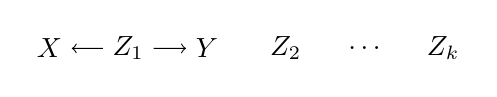
\begin{tikzpicture}[yscale=.75]
				\node (x) at (0,1) {$X$};
				\node (y) at (2,1) {$Y$};
				\node (z) at (1,1) {$Z_1$};
				\node at (3,1) {$Z_2$};
				\node at (4,1) {$\ldots$};
				\node at (5,1) {$Z_k$};
				\draw [->] (z) -- (y);
				\draw [->] (z) -- (x);
				\end{tikzpicture}
			\end{figure}
			\begin{equation*}
				\begin{split}
					\bm{z_1} &= Binom(1, 0.5) \\
					\bm{x} &= Binom(1, \bm{z_1} / 3) \\
					\bm{y} &= Binom(1, \bm{z_1} / 3) \\
					\bm{z_i} &= Uniform([0, 1]) \forall i \in \{ 2, \cdots, k \} \\
				\end{split}
			\end{equation*}
	\end{itemize}
\end{frame}

\begin{frame}
	\frametitle{Empirical Analysis: Calibration}
	\begin{figure}
		\centering
		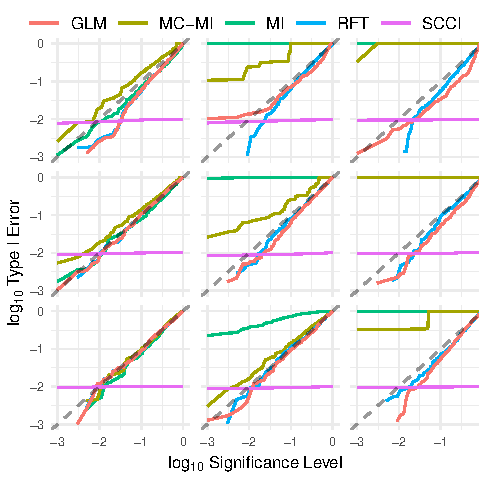
\includegraphics[scale=0.8]{imgs/calibration_add_vars.pdf}
		\caption*{Type I error vs significance level for varying sample sizes (top to
		bottom): $ [20, 40, 80] $ and number of conditional variables (left to
		right): $ [1, 3, 5] $}
	\end{figure}
\end{frame}

\begin{frame}
	\frametitle{Empirical Analysis: Discrimination Data generation}
	\begin{itemize}
		\item When the null hypothesis is false, the test should be able to reject the null i.e. should have power.
		\item We test the accuracy of correctly classifying datasets as conditionally dependent or independent.
		\item Dependent datasets are generated with varying effect strength for $ X \to Y $: 
			\begin{figure}
					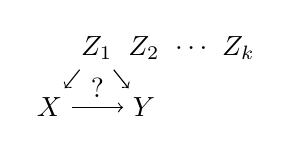
\begin{tikzpicture}[yscale=.75, xscale=.6]
						\node (x) at (0,0) {$X$};
						\node (y) at (2,0) {$Y$};
						\node (z) at (1,1) {$Z_1$};
						\node at (2,1) {$Z_2$};
						\node at (3,1) {$\ldots$};
						\node at (4,1) {$Z_k$};
						\draw [->] (x) edge node [midway, above] {?} (y);
						\draw [->] (z) -- (y);
						\draw [->] (z) -- (x);
					\end{tikzpicture}
			\end{figure}
		\item Binary data is generated using the logistic model: 
			\begin{equation*}
				p( y_i = 1 ) = \lambda\left( \sum_{X \text{ is a parent of } Y} \beta x_i \right) ; \lambda(x) = \frac{e^x}{e^x + 1}
			\end{equation*}
		\item Independent datasets are generated by setting the effect to $ 0 $.
	\end{itemize}
\end{frame}

\begin{frame}
	\frametitle{Empirical Analysis: Discrimination}
	\begin{figure}
		\centering
		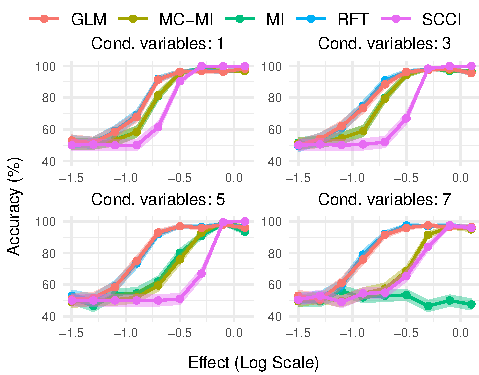
\includegraphics{imgs/accuracy.pdf}
		\caption*{Accuracy (shading: mean $\pm$ standard error, $N=200$)
		of classifying simulated binary datasets (sample size: $1000$)
		as conditionally dependent or independent.}
	\end{figure}

\end{frame}

\begin{frame}
	\frametitle{Epirical Analysis: Discrimination Data Generation (Ordinal)}
	\begin{itemize}
		\item Same as the last analysis but ordinal datasets are used.
		\item Conditionally independent data with $ k = 8 $ levels are generated as:
			\begin{equation*}
				\begin{split}
					z_i &= \textit{Binom}(k-1, 0.5) \\
					x &= \textit{Binom}(k-1, z_1/k) \\
					y &= \textit{Binom}(k-1, z_1/k) \\
				\end{split}
			\end{equation*}
		\item For conditionally dependent data, $ z_1 $ is randomly permuted.
	\end{itemize}
\end{frame}

\begin{frame}
	\frametitle{Empirical Analysis: Discrimination (Ordinal)}
	\begin{figure}
		\centering
		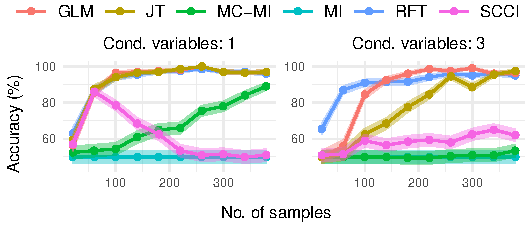
\includegraphics{imgs/accuracy_ordinal.pdf}
		\caption*{Accuracy (shading: mean $\pm$ standard error) of
		classifying simulated ordinal data (8 levels per variable) as
		conditionally dependent or independent.}	
	\end{figure}
\end{frame}

\begin{frame}
	\frametitle{Applications: Model testing Data generation}
	\begin{itemize}
		\item Given a DAG and a dataset, how well is the test able to
			detect the implied CIs of the DAG in a given dataset.
		\item We generate random DAGs on 20 variables with varying edge density.
		\item We then simulate data (sample size of $1000 $) from the
			DAGs using logistic regression and a fixed effect of
			0.15 for all edges.
		\item We use the CI tests to test all the implied CIs and an equal number of 
			randomly generated CIs in the simulated dataset.
	\end{itemize}
\end{frame}

\begin{frame}
	\frametitle{Applications: Model testing}
	\begin{figure}
		\centering
		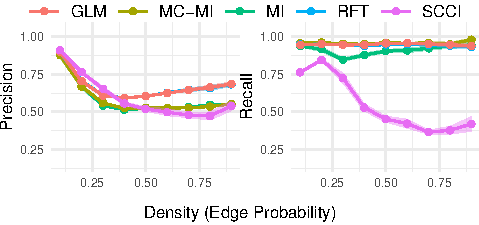
\includegraphics{imgs/model_testing.pdf}
		\caption*{Precision and recall (shading: mean $\pm$ standard
		error) of testing implied CIs and equal number of randomly
		generated CIs in binary datasets}
	\end{figure}
\end{frame}

\begin{frame}
	\frametitle{Applications: Structure Learning data generation}
	\begin{itemize}
		\item Test how well is the test able to recover a DAG from given dataset.
		\item Generated random DAGs on 20 variables with varying the edge probability.
		\item We then simulate data (sample size of $1000 $) from the
			DAGs using logistic regression and a fixed effect of
			0.15 for all edges.
		\item PC algorithm (stable variant) is used to learn the DAG back from the simulated datasets.
		\item F1-Score is computed for comparing the true and the learnt edges.
	\end{itemize}
\end{frame}

\begin{frame}
	\frametitle{Applications: Structure Learning}
	\begin{figure}
		\centering
		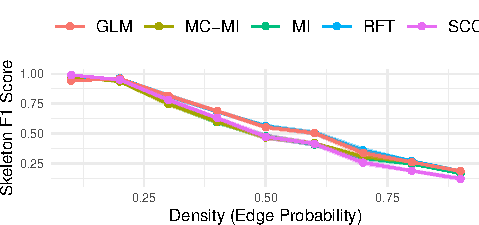
\includegraphics{imgs/sl_density.pdf}
		\caption*{F1-score
		(shading: mean $\pm$ standard error) of the learned model
		skeletons.}
	\end{figure}
\end{frame}

\begin{frame}
	\frametitle{Applications: Structure Learning}
	\begin{figure}
		\centering
		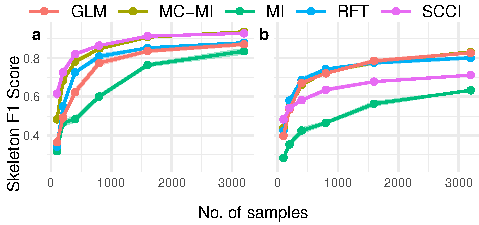
\includegraphics{imgs/sl.pdf}
		\caption*{Structure learning on (a) ``alarm'', and (b)
		``insurance'' datasets.  F1-score (shading: mean $\pm$ standard
		error, $N=10$) of the learned model skeletons.}
	\end{figure}
\end{frame}

\begin{frame}
	\frametitle{Applications: Structure Learning}
	\begin{figure}
		\centering
		\begin{subfigure}{0.5\textwidth}
			\centering
			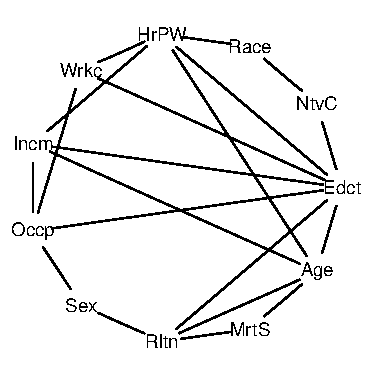
\includegraphics[scale=0.85]{imgs/sl-adult-rf.pdf}
			\caption*{}
			\label{fig:sl_adult_model}
		\end{subfigure}%
		\begin{subfigure}{0.5\textwidth}
			\centering
			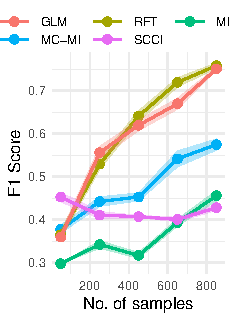
\includegraphics{imgs/adult_F1.pdf}
			\caption*{}
			\label{fig:sl_adult}
		\end{subfigure}
		\caption*{Structure learning on US census income dataset. (a)
		Learnt skeleton using RFT. (b) F1-score (shading: mean $\pm$
		standard error, $N=10$) when comparing $d$-connected variable
		pairs from the CPDAG to correlated variable pairs in the
		dataset.}
	\end{figure}
\end{frame}

\begin{frame}
	\frametitle{Runtime Analysis}
	\begin{figure}
		\centering
		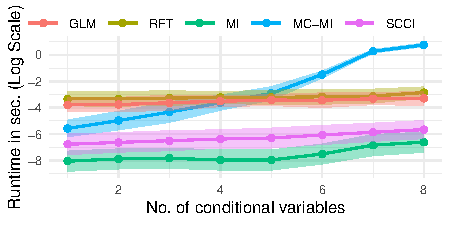
\includegraphics{imgs/runtime.pdf}
		\caption*{Runtime (shading: mean $\pm$ standard error, $N=100$)
		for CI tests with varying numbers of conditional variables and
		$1000$ samples per dataset.
		}
	\end{figure}
\end{frame}

\section{Conclusion}
\begin{frame}
	\frametitle{Conclusion/Future Work}
	\begin{itemize}
		\setlength\itemsep{1em}
		\item A residualization based CI test that works for a combination of ordinal and categorical variables.
		\item Properties: 1) Simple to implement; 2) Interpretable chi-square test statistic; 3) Symmetric by construction; 4) Computationally feasible
		\item Performs reasonably well for low number of
			conditional variable but performs better for high
			number of conditional variables.
		\item For structure learning, a hybrid approach can be used with other
			tests.
		\item Estmiators like Random Forests can work with combination of discrete and 
			continuous variables, can possibly be extended to a single 
			unified test for all data types.
	\end{itemize}
\end{frame}

\begin{frame}
	\begin{center}
		\Huge{Questions}
	\end{center}
	\begin{center}
		Paper preprint: https://arxiv.org/pdf/2206.04356.pdf
	\end{center}
\end{frame}

\end{document}
